


\section{Introduction}
In perovskite solar cells, the absorber is usually sandwiched between two different contacts: the \gls{htm} and the \gls{etm}, with the role of extracting respectively the positive and negative free charges.
Without this asymmetrical extraction of charges, the photogeneration would be of no use.
The classical \gls{etm} from \gls{dssc}, mesoporous titania, is getting obsoleted by planar tin oxide \cite{Jiang2018}.
On the contrary, the classical \gls{htm} from solid-state \gls{dssc}, \gls{spiro}, is still present in most of the record structures of \gls{csfamapbibr} based solar cells \cite{Saliba2016,Saliba2018}.
The huge explorative work done for finding a better performing \gls{htm} managed to find very few good alternatives.% small molecules or polymers (\textsl{e.g.} \gls{ptaa}).
Still, even if the performances are at par with \gls{spiro}, the commercial price of these alternative \gls{htm} is still too high for wide area applications.
A better understanding of the \gls{htm}\-/perovskite interaction is needed for pinpointing the key characteristics to be looked for in the next \gls{htm} design.
In this chapter, the devices fabricated using four different \gls{htm}, including two novel ones: \gls{tae3} and \gls{tae4}, have been compared in order to find a correlation with the \gls{htm}'s chemical properties.
The devices have been fabricated by me under the supervision of Dr.\ Nuria F.\ Montcada and Prof.\ Emilio J.\ Palomares Gil (fabrication described in \cpagerefrange{methods_bottom}{methods_bottom_end}).
The current\hyp{}voltage sweeps characterization was performed by me and NFM.
The transient electronic characterization was performed and analysed by me using equipment built by Dr.\ Javier Pérez Hernández.
The electrochemical and optical characterization of the molecules was performed by NFM, Dr.\ Lydia Cabau, Dr.\ Agustín Molina Ontoria, and Dr.\ Inés García\hyp{}Benito.
Molecular simulations have been performed by Prof.\ Anton Vidal\hyp{}Ferran.
Dr.\ Agustín Molina Ontoria and Prof. Nazario Martín designed \gls{tae1} (CAS 1802982-22-4, after the first report in \cite{Cabau2015a}, it has been used also by other research groups in \cite{Choi2015b,Labban2016,Wu2016a,Wu2016b}), \gls{tae3} (CAS 2055756-83-5), and \gls{tae4} molecules.
The synthesis of these has been carried on by Dr.\ Inés García\hyp{}Benito and reported in her PhD thesis \cite{Garcia-Benito2017} (there, \gls{tae3} is labelled as BF-1, and \gls{tae4} as BF-2) and in \cite{Gelmetti2019}.
Further characterization of the workfunction of the \gls{htm} surface when layered on top of \gls{fto} or \ch{TiO2} or \gls{csfamapbibr} has been performed using \gls{kpfm} by Dr.\ Ana Pérez-Rodríguez, Dr.\ Esther Barrena, and Prof.\ Carmen Ocal at ICMAB-CSIC, UAB, Barcelona.
The measured \gls{cpd} allowed us to study the impact the underlying perovskite layer can have on the \gls{htm} material.
These measurements have been discussed in Dr.\ Ana Pérez-Rodríguez PhD thesis \cite{Perez-Rodriguez2018}.

\begin{figure}
	\makebox[\textwidth][c]{
		\parbox{1.1\textwidth}{
			\centering
			\begin{subfigure}[t]{0.51\textwidth}
								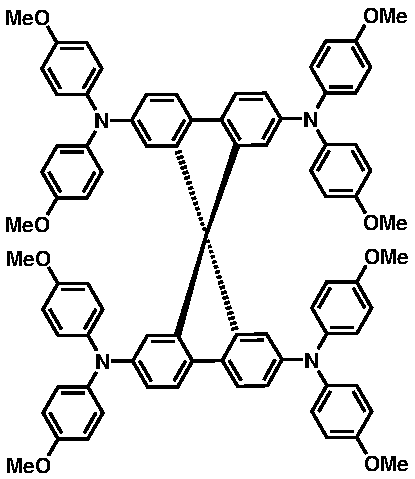
\includegraphics[scale=0.8]{molecules/spiro.pdf}
				\subcaption{\gls{spiro}}\label{fig:tae-molecules-spiro}
			\end{subfigure}
			\qquad
			\begin{subfigure}[t]{0.51\textwidth}
								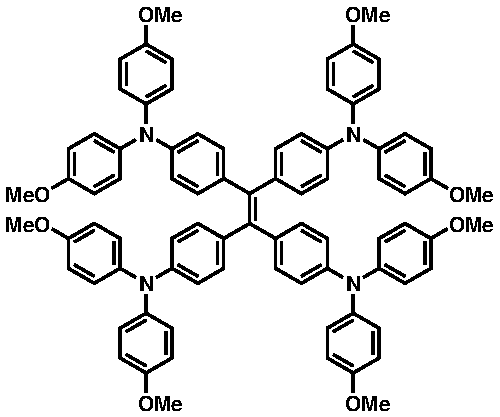
\includegraphics[scale=0.8]{molecules/tae1.pdf}
				\subcaption{\gls{tae1}}\label{fig:tae-molecules-tae1}
			\end{subfigure}
			\bigskip
			
			\begin{subfigure}[t]{0.51\textwidth}
				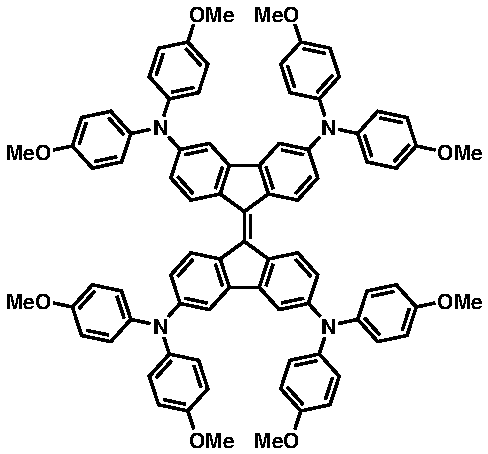
\includegraphics[scale=0.8]{molecules/tae3.pdf}
				\subcaption{\gls{tae3}}\label{fig:tae-molecules-tae3}
			\end{subfigure}
			\qquad
			\begin{subfigure}[t]{0.51\textwidth}
				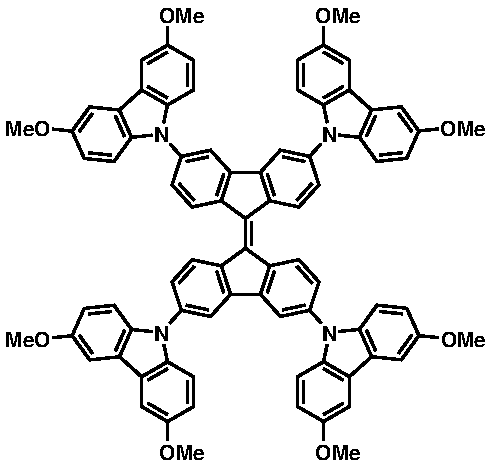
\includegraphics[scale=0.8]{molecules/tae4.pdf}
				\subcaption{\gls{tae4}}\label{fig:tae-molecules-tae4}
			\end{subfigure}
			\mycaption[Chemical structures of HTM utilised for bottom cathode solar cells.]{}\label{fig:tae-molecules}
		}
	}
\end{figure}

\section{Design of the Experiment}
In order to compare different materials for the selective contact layer, we decided to avoid any modification to the layers underlying the absorber one in the solar cell stack, as these could heavily affect the perovskite morphology \cite{Tao2017}.
%The variation of the upper contact (\textsl{i.e.} the \gls{htm} in bottom cathode solar cells) guarantees that the observed differences will not be due to a different perovskite structure, whose crystallization has been reported to be sensible to the underlying contact 
Additionally, the \gls{htm} under comparison have been deposited under as similar as possible conditions (partially hindered by a different solubility), employing the same additives and thicknesses.
For reducing the possible \gls{dos} width differences for different molecules, the chosen \gls{htm} have all very similar chemical structures.

%
Solvent annealing of contact Wu2016

Energy disorder Shao2016

HOMO shift measured by CE and DC has been correlated with UPS for OSC Credgington2014
%
%Steepness of absorbance onset also indicates the presence/absence of mid-gap states in the HTM, whose presence would favour the surface recombination \cite{Tvingstedt2017}
%
%Impact of dopants in HTM on voc \cite{Correa-Baena2017} "Therefore, dopants act as recombination centers at the HSL interface and dominate recombination dynamics over e.g. the energetics of the HTM which is secondary as shown in a recent study by Belisle et al.39"
%
%"the often-questionable validity of vacuum level alignment, the importance of interface dipoles, and band bending as the result of interface formation" \cite{Schulz2019}
%

\section{Stored charge profile analysis}

\section{Recombination analysis}

%\section{Layers workfunction \textit{via} KPFM}
%\section{Conclusions}
%\section{Critical Assessment}

